\chapter{Results}
\label{chap:tables}

Chapters containing experimental results often contain a number of
tables.  These are ``floated'' in \LaTeX, just like figures.  The
short caption is automatically added to the ``List of Tables'' page,
and---like a figure---the table can contain almost anything
(graphics, text, tabular material, code snippets or whatever).

The most important thing to establish is the difference between
the {\tt table} and {\tt tabular} environments.  A table is just a
floating body, but the tabular environment is used to create
{\em actual} tables.  The following examples show what you can do with
both environments.

\section{The {\tt table} Environment}

Table~\ref{tab:ex1} is an example of a table with graphical content.
Note one convention:  unlike figures, tables are usually captioned at
the {\bf top}, not the bottom.  

As with figures, the best place to put the \verb|\label| is directly
after the \verb|\caption|, otherwise you will end up with the section
label instead.  You can find the code for Table ~\ref{tab:ex1} on page~42,
starting at line~106.

\section{The {\tt tabular} Environment}

Most likely what you will want to put inside a {\tt table} environment
is a table of data.  This is done using the {\tt tabular} environment,
as in the following example.  This code:

\linespread{1}\small
\begin{quote}
\begin{verbatim}
\begin{tabular}{l|c|c}
Day & Cups of Coffee & Lines of Code \\
\hline
Mon & 3 & 200 \\
Tue & 5 & 500 \\
Wed & 5 & 300 \\
Thu & 4 & 200 \\
Fri & 3 & 100 \\
\end{tabular}
\end{verbatim}
\end{quote}
\linespread{1.3}\normalsize

will produce this table:

\begin{center}
\begin{tabular}{l|c|c}
Day & Cups of Coffee & Lines of Code \\
\hline
Mon & 3 & 200 \\
Tue & 5 & 500 \\
Wed & 5 & 300 \\
Thu & 4 & 200 \\
Fri & 3 & 100 \\
\end{tabular}
\end{center}

The vertical bars in the \verb+{l|c|c}+ argument tell \LaTeX\ to put
lines between each column. The argument \verb+{|l|c|c|}+ would have
resulted in lines around the outside as well. The letters indicate the
text formatting in the table (l for left, c for center, etc.).  The
command \verb|\hline| is used to add horizontal lines (including at
the top and bottom of the table) and \verb|\\| is used to end each
row.  You do not need to use \verb|\\| at the end of \verb|\hline|.
Finally, the {\tt \&} character is used to separate entries within
rows.

Table~\ref{tab:ex2} is a slightly more complex example of tabular
material, included as a table in the document.  Here is the code which
produced it:

\linespread{1}\small
\begin{quote}
\begin{listing}{1}
\begin{table}
\hrulefill
\caption[A tabular table]{An example of a table whose contents are
formatted using the {\tt tabular} environment.}
\label{tab:ex2}
\hrulefill
\begin{center}
\begin{tabular}{|l|l|r|} \hline\hline
{\em type} & \multicolumn{2}{c|}{\em style} \\ \hline
smart & red & short \\
rather silly & puce & tall \\ \hline\hline
\end{tabular}
\end{center}
\par
\bigskip
\hrulefill
\end{table}
\end{listing}
\end{quote}
\linespread{1.3}\normalsize

The \verb|\multicolumn| command on line 8 allows the spread of data
over several columns, and overrides the normal vertical bar placement.
Lines 2, 6 and 14--16 produce the horizontal lines which separate
the table from the rest of the text.

\begin{table}
\hrulefill
\caption[A table with graphical input]{An example of a table which
uses graphical input as its content.  This is once again the
contents page of this document, saved as PDF.}
\label{tab:ex1}
\hrulefill
\begin{center}
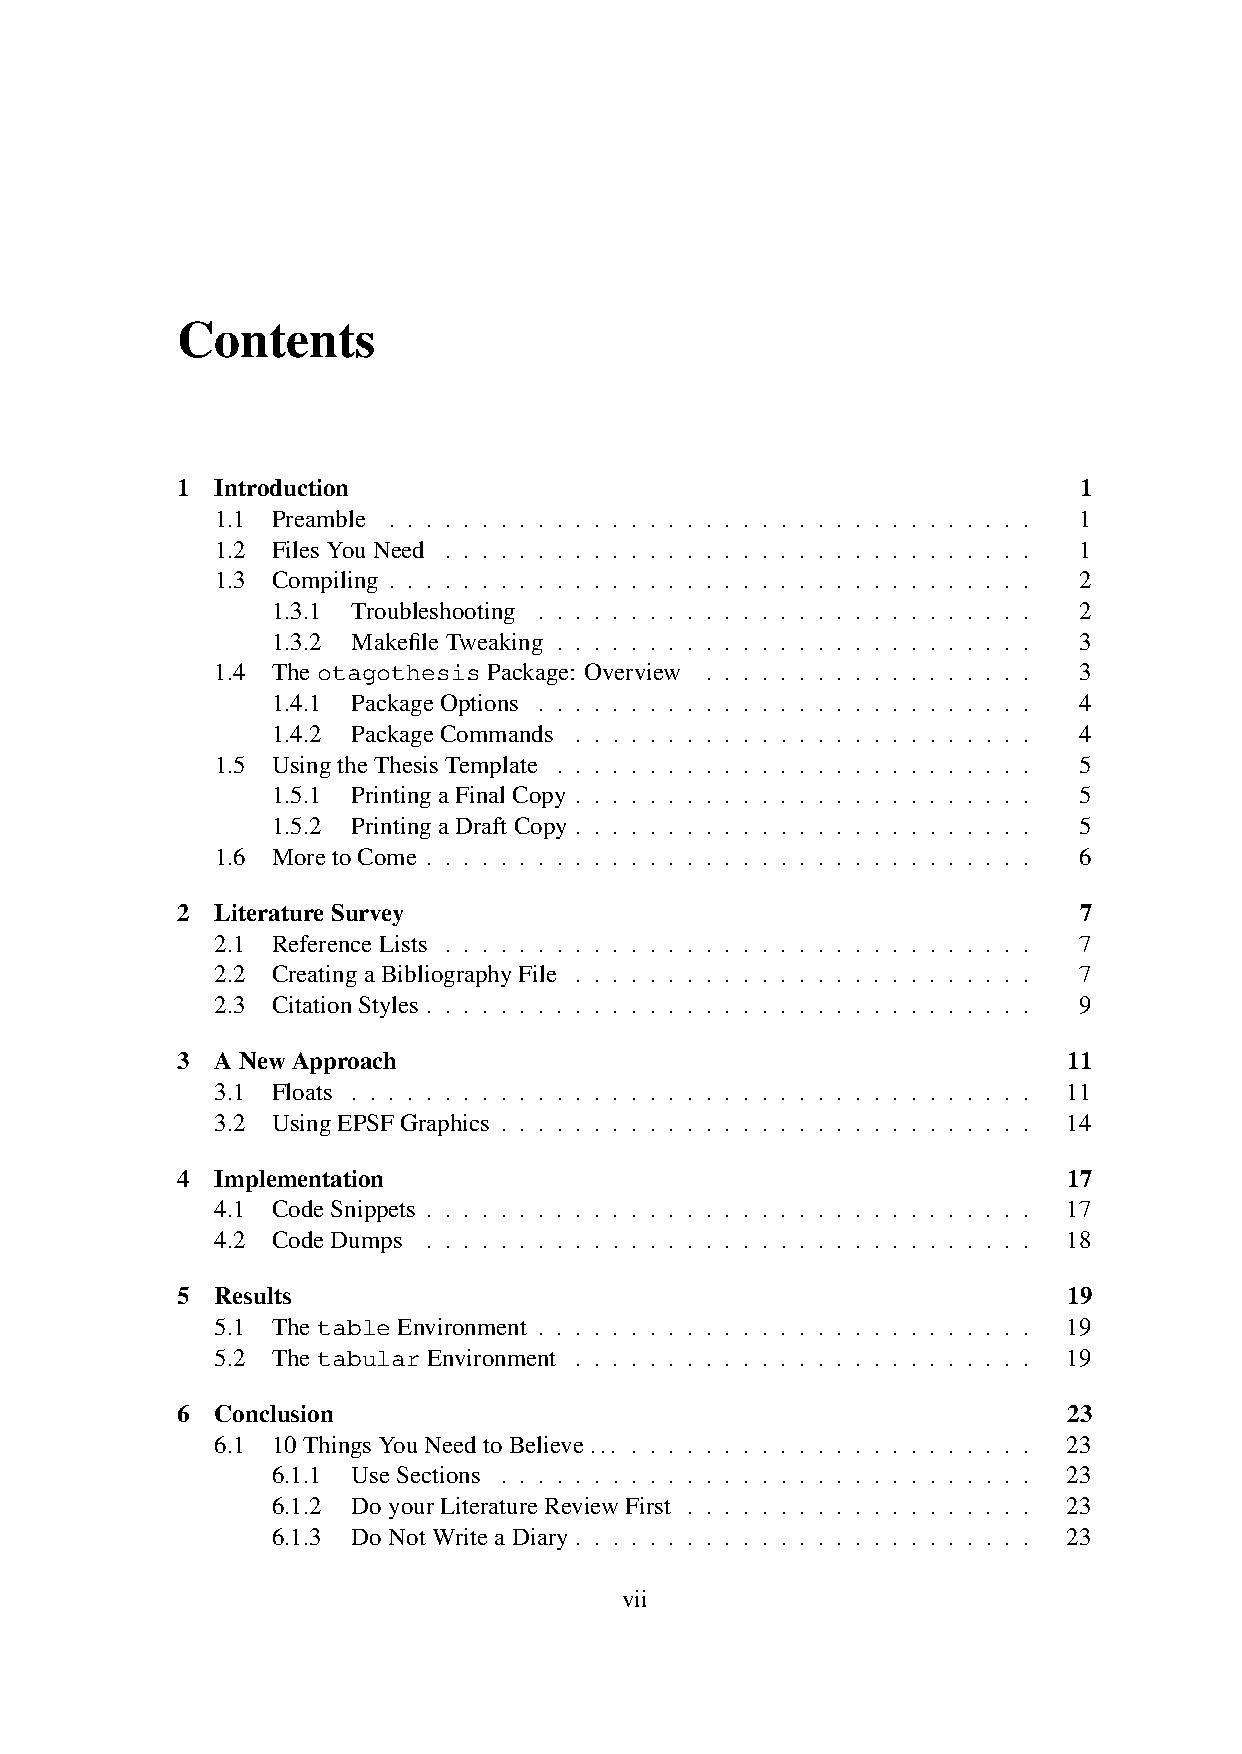
\includegraphics[scale = 0.5, angle = 270]{page.pdf}
\end{center}
\par
\bigskip
\hrulefill
\end{table}


\begin{table}
\hrulefill
\caption[A tabular table]{An example of a table whose contents are
formatted using the {\tt tabular} environment.}
\label{tab:ex2}
\hrulefill
\begin{center}
\begin{tabular}{|l|l|r|}
\hline\hline
{\em type} & \multicolumn{2}{c|}{\em style} \\ \hline
smart & red & short \\
rather silly & puce & tall \\ \hline\hline
\end{tabular}
\par
\bigskip
\hrulefill
\end{center}
\end{table}
